\documentclass{article}
\usepackage{amsmath}
\usepackage{mathtools}
\usepackage{gensymb}
\usepackage[a4paper,inner=1.5cm,outer=1.5cm,top=2cm,bottom=0.5cm]{geometry} 
\usepackage{xcolor}                    
\usepackage{tikz}                           
\usepackage{multicol}
\usepackage{pgfplots}
\usetikzlibrary{calc}
\usetikzlibrary{intersections}
\usetikzlibrary{intersections,calc,angles,quotes}
\usetikzlibrary{shapes,arrows,positioning,decorations.pathreplacing,calc}
\usetikzlibrary{calc,angles,positioning,intersections,quotes,decorations.markings}
\usepackage{tkz-euclide}
\usetikzlibrary{backgrounds}
\usetikzlibrary{calc,through}
\usetikzlibrary{angles}
\usetikzlibrary{fadings}
\usetikzlibrary{shapes.geometric}
\usetikzlibrary{shapes.symbols}
\usepackage{draftwatermark}
\usepackage{mathptmx}

\SetWatermarkText{\textcolor{black!30}{Mathema Shukur}}
\SetWatermarkFontSize{2 cm}
\usepackage[utf8]{inputenc}
\usepackage{fontspec}

\setmainfont{[Kalpurush.ttf]}
\newfontface{\en}{[Arial.ttf]} %%this is optional, if you want to use a secondary font. Any english font is supported
\newlength\Radius
\setlength\Radius{4cm}
\begin{document} 
	\Large
	\textcolor{red}{Welcome To} 
	\\
	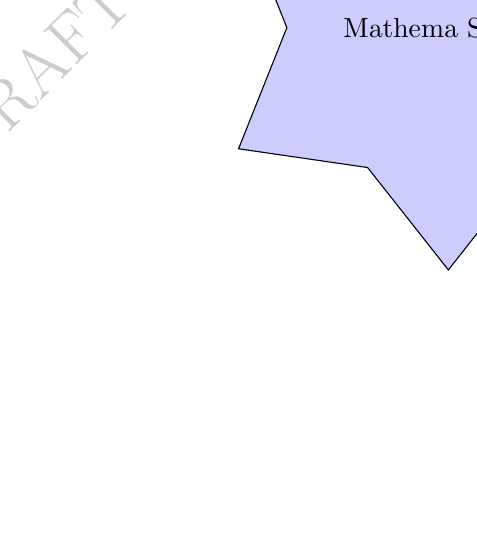
\begin{tikzpicture}
		\tikz \node [fill=blue!20,star,star points=6,draw] {Mathema Shukur };
	\end{tikzpicture}
	\\
	যাদের জন্যে প্রযোজ্যঃ  	\textcolor{magenta}{একাদশ ও দ্বাদশ শ্রেণীর শিক্ষার্থী} \\
	বিষয়ঃ \textcolor{magenta}{উচ্চতর গণিত ১ম পত্র} \\
	অধ্যায়ঃ \textcolor{magenta}{৩-সরলরেখা}\\ 
	Subtopicঃ  \textcolor{magenta}{  সরলরেখার বিভিন্ন আকারের সমীকরণ নির্ণয় করা   }\\
	\\
	\textcolor{blue}{(1)	ঢাল বিন্দু আকার Point slope form}\\
	\\
	$(y-y_1)=m(x-x_1)$\\
	\\
	\textcolor{red} {(2)  দুই বিন্দু আকার 	Two point form}\\
	\\
	$y-y_1=\left(\frac{y_1-y_2}{x_1-x_2}\right)(x-x_1)$\\
	\\
	\textcolor{green}{ (3) ঢাল খণ্ডন আকার 	Slope intercept form}\\
	\\
	$y=mx+c$\\
	\\
	\textcolor{cyan}{ (4) দ্বি খণ্ডন আকার  Two	Intercept form}\\
	\\
	$\frac{x}{a}+\frac{y}{b}=1$\\
	\\
	\\
	\textcolor{purple}{ (5) লম্ব  আকার  Normal form}\\
	\\
	মূল বিন্দু হতে কোনো সরলরেখার উপর অঙ্কিত লম্বের দৈর্ঘ্য $p$ এবং লম্বটি $x-$ অক্ষের ধনাত্মক দিকের সাথে $\alpha$ কোণ উৎপন্ন করলে, রেখাটির সমীকরণ নির্ণয় কর \\ 
	\\
	$x\cos \alpha +y\sin \alpha=p$\\
	\\
	\\
	\textcolor{olive}{ (6) সাধারণ  আকার  General form}\\
	\\
	$ax+by+c=0$\\
	\\
		\\
	\textcolor{magenta}{ (7) ছেদবিন্দু অতিক্রমণ  আকার  Through intersection  form}\\
	\\
 দুইটি সরলরেখা 	$a_1x+b_1y+c_1=0$ ও  $a_2x+b_2y+c_2=0$ এর ছেদবিন্দু গামী রেখার সমীকরণ \\
 \\
	$(a_1x+b_1y+c_1)+k(a_2x+b_2y+c_2)=0$\\
	\\
	$k$ ইচ্ছাধীন ধ্রুবক তবে শূন্য নয় \\ 
	\\
	(একটি সরলরেখা ) $+k$ (অপর সরল রেখা) $=0$\\
	\\ 
	ঢাকা বোর্ড-২০১৯\\ 
	$x+y=2$ এবং  $y-x=0$ রেখাদ্বয়ের ছেদবিন্দুগামী এবং  $x-$ অক্ষের সমান্তরাল রেখার সমীকরণ নির্ণয় কর \\
	\\
	যেকোনো অশূন্য ধ্রুবক $k$ এর ক্ষেত্রে $x+y=2$ এবং  $y-x=0$ রেখাদ্বয়ের ছেদবিন্দুগামী  রেখার সমীকরণ 
	\begin{align*}
		(x+y-2)+k(y-x)&=0\\
		\\
		x+y-2+ky-kx&=0\\
		\\
		(1-k)x+(1+k)y-2&=0
	\end{align*}
\\ 
রেখাটি $x-$ অক্ষের সমান্তরাল হলে $x$ এর সহগ শূন্য হবে \\ 
\\
	$1-k=0$,\qquad $k=1$\\
	\\  
		\begin{align*}
		(1-k)x+(1+k)y-2&=0\\
		(1-1)x+(1+1)y-2&=0\\
		2y-2&=0\\
		y-1&=0\\
	\end{align*}
\\
		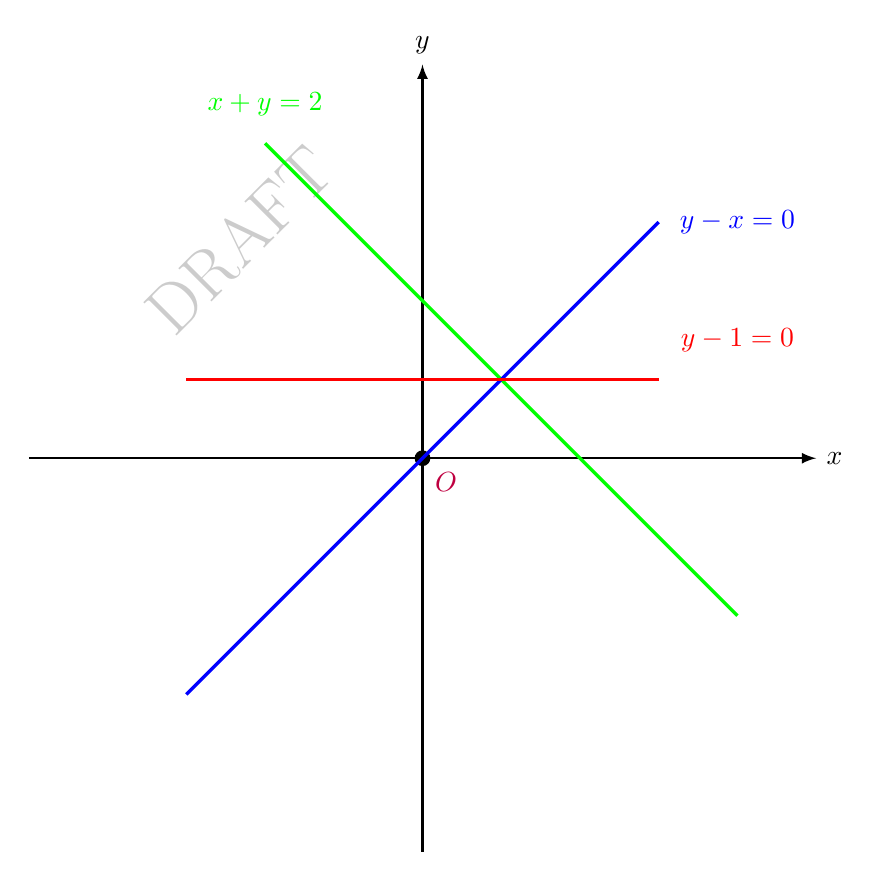
\begin{tikzpicture}[transform shape,scale=1]
		\draw [-latex,thick](-5,0) -- (5,0) node[right] {$x$} coordinate(x axis);
		\draw [-latex,thick](0,-5) -- (0,5) node[above] {$y$} coordinate(y axis);
		\fill[black] (0,0) circle (1 mm);
		\node at (0.3,-0.3) {$\textcolor{purple}{O}$};	
		\node at (4,3) {$\textcolor{blue}{y-x=0}$};	
		\node at (-2,4.5) {$\textcolor{green}{x+y=2}$};
		\node at (4,1.5) {$\textcolor{red}{y-1=0}$};		
		\draw[very thick,green] (-2,4)--(4,-2);	
		\draw[very thick,blue] (3,3)--(-3,-3);	
			\draw[very thick,red] (-3,1)--(3,1);	
	\end{tikzpicture}
\\
	সকল বোর্ড-২০১৮\\
		$x+y=5$ এবং  $y-x=3$ রেখাদ্বয়ের ছেদবিন্দুগামী এবং  $y-$ অক্ষের সমান্তরাল রেখার সমীকরণ নির্ণয় কর \\
	\\
		যেকোনো অশূন্য ধ্রুবক $k$ এর ক্ষেত্রে 	$x+y=5$ এবং  $y-x=3$ রেখাদ্বয়ের ছেদবিন্দুগামী রেখার সমীকরণ 
	\begin{align*}
		(x+y-5)+k(y-x-3)&=0\\
		\\
		x+y-5+ky-kx-3k&=0\\
		\\
		(1-k)x+(k+1)y-3k-5&=0
	\end{align*}
\\ 
রেখাটি $y-$ অক্ষের সমান্তরাল হলে $y$ এর সহগ শূন্য হবে \\ 
\\
$k+1=0$,\qquad $k=-1$\\
\\ 
	\begin{align*}
	(1-k)x+(k+1)y-3k-5&=0\\
	(1-(-1))x+(-1+1)y-3(-1)-5&=0\\
	2x-2&=0\\
	x-1&=0
\end{align*}
\\ 
	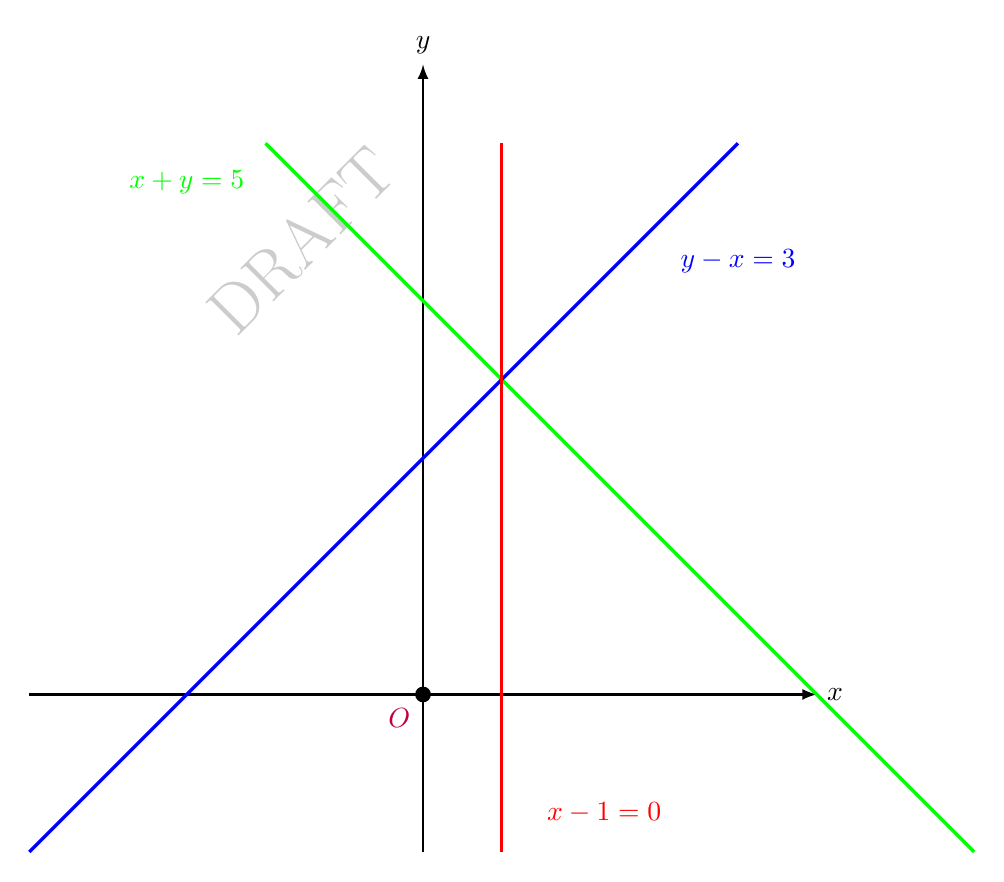
\begin{tikzpicture}[transform shape,scale=1]
		\draw [-latex,thick](-5,0) -- (5,0) node[right] {$x$} coordinate(x axis);
		\draw [-latex,thick](0,-2) -- (0,8) node[above] {$y$} coordinate(y axis);
		\fill[black] (0,0) circle (1 mm);
		\node at (-0.3,-0.3) {$\textcolor{purple}{O}$};	
		\node at (4,5.5) {$\textcolor{blue}{y-x=3}$};	
		\node at (-3,6.5) {$\textcolor{green}{x+y=5}$};
		\node at (2.3,-1.5) {$\textcolor{red}{x-1=0}$};		
		\draw[very thick,green] (-2,7)--(7,-2);	
		\draw[very thick,blue] (4,7)--(-5,-2);	
		\draw[very thick,red] (1,-2)--(1,7);	
	\end{tikzpicture}
	\\
		চট্রগ্রাম বোর্ড-২০১৭\\
	$x+y=6$ এবং  $y-x=2$ রেখাদ্বয়ের ছেদবিন্দুগামী এবং  $x-$ অক্ষের উপর লম্ব রেখার সমীকরণ নির্ণয় কর \\
		\\
	ঢাকা বোর্ড-২০১৩\\
$x-$ অক্ষের সমান্তরাল এবং  $4x+3y=6$ ও $x-2y=7$রেখা দুইটির সমবিন্দু সরলরেখার সমীকরণ নির্ণয় কর \\
	\\
		যেকোনো অশূন্য ধ্রুবক $k$ এর ক্ষেত্রে  $4x+3y=6$ ও $x-2y=7$রেখা দুইটির সমবিন্দু সরলরেখার সমীকরণ
	\begin{align*}
		(4x+3y-6)+k(x-2y-7)&=0\\
		\\
		4x+3y-6+kx-2ky-7k&=0\\
		\\
		(k+4)x+(3-2k)y-7k-6&=0
	\end{align*}
\\ 
রেখাটি $x-$ অক্ষের সমান্তরাল হলে $x$ এর সহগ শূন্য হবে \\ 
\\
$k+4=0$,\qquad $k=-4$\\
	\\
\begin{align*}
	(k+4)x+(3-2k)y-7k-6&=0\\
	\\
	(-4+4)x+(3-2(-4))y-7(-4)-6&=0\\
	\\
	11y+28-6&=0\\
	\\
	11y+22&=0\\
	\\
	y+2&=0 
\end{align*}
\\ 
		\begin{tikzpicture}[transform shape,scale=1]
		\draw [-latex,thick](-4,0) -- (9,0) node[right] {$x$} coordinate(x axis);
		\draw [-latex,thick](0,-6) -- (0,6) node[above] {$y$} coordinate(y axis);
		\fill[black] (0,0) circle (1 mm);
		\node at (-0.3,-0.3) {$\textcolor{purple}{O}$};	
		\node at (9,1.5) {$\textcolor{green}{x-2y=7}$};	
		\node at (-3,6.5) {$\textcolor{blue}{4x+3y=6}$};
		\node at (8,-2.5) {$\textcolor{red}{y+2=0}$};		
		\draw[very thick,green] (-3,-5)--(9,1);	
		\draw[very thick,blue] (-3,6)--(6,-6);	
		\draw[very thick,red] (-4,-2)--(8,-2);	
	\end{tikzpicture}
\end{document}